% ---------------------------------------------------------------------------- %
\begin{figure}
	\centering
	\subfigure[\label{fig:linguometer:architecture:sig:lmwords:1}]
	{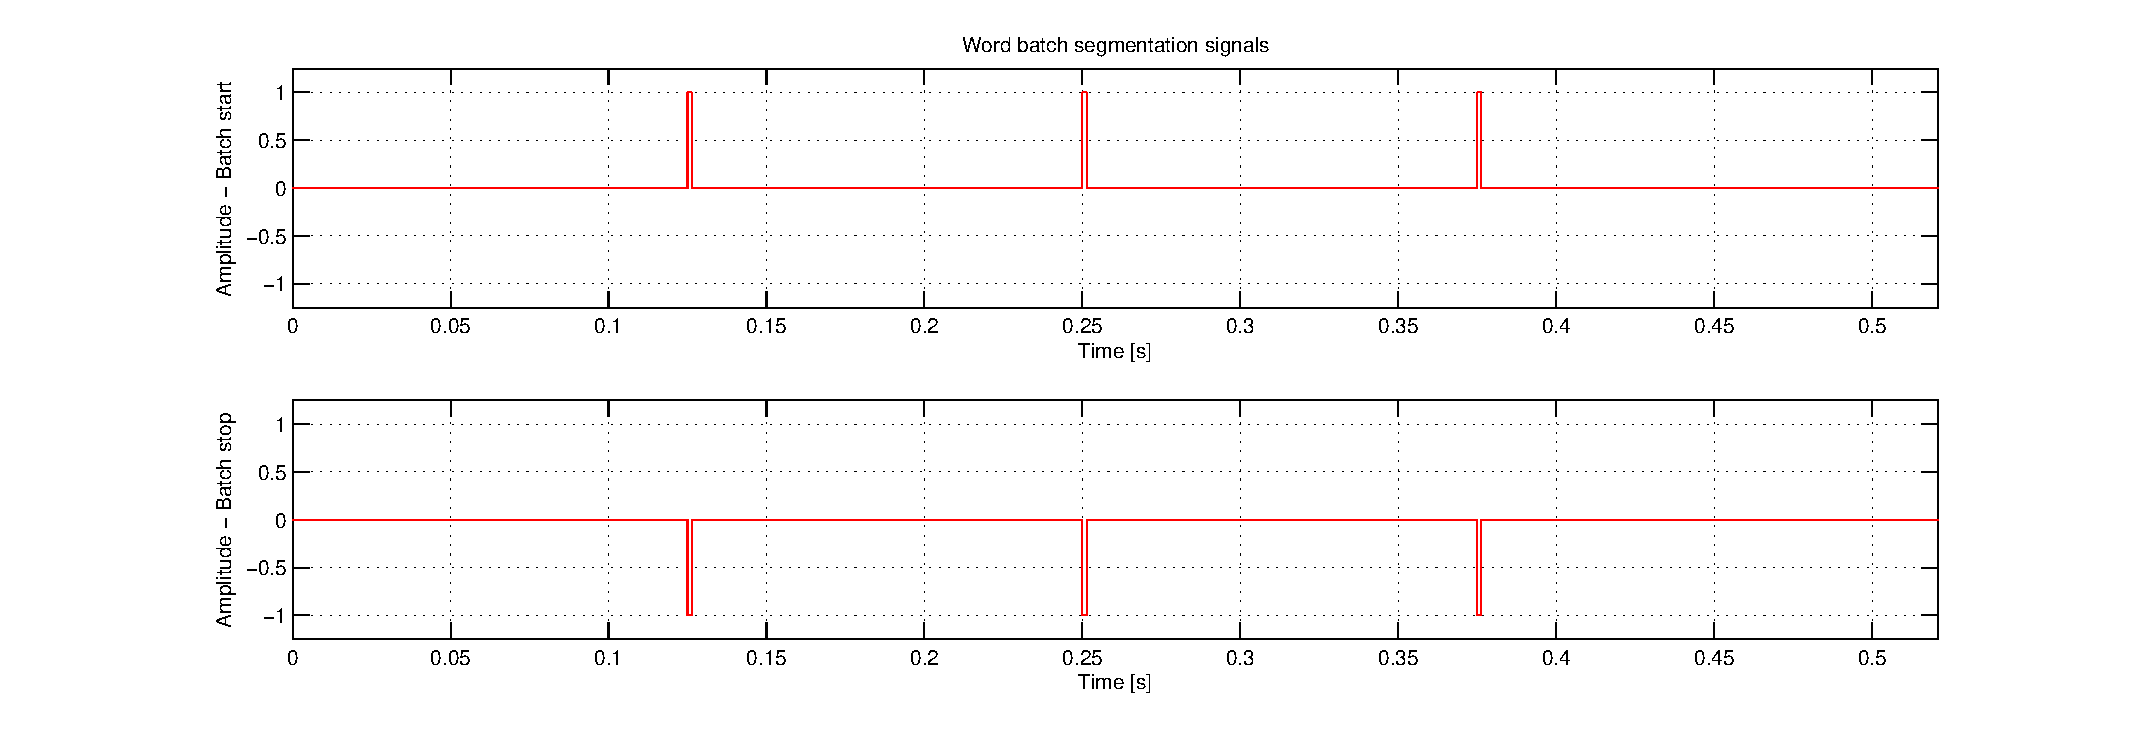
\includegraphics[width=\textwidth]{include/linguometer/images/seg_batch.eps}}
	
	\subfigure[\label{fig:linguometer:architecture:sig:lmwords:2}]
	{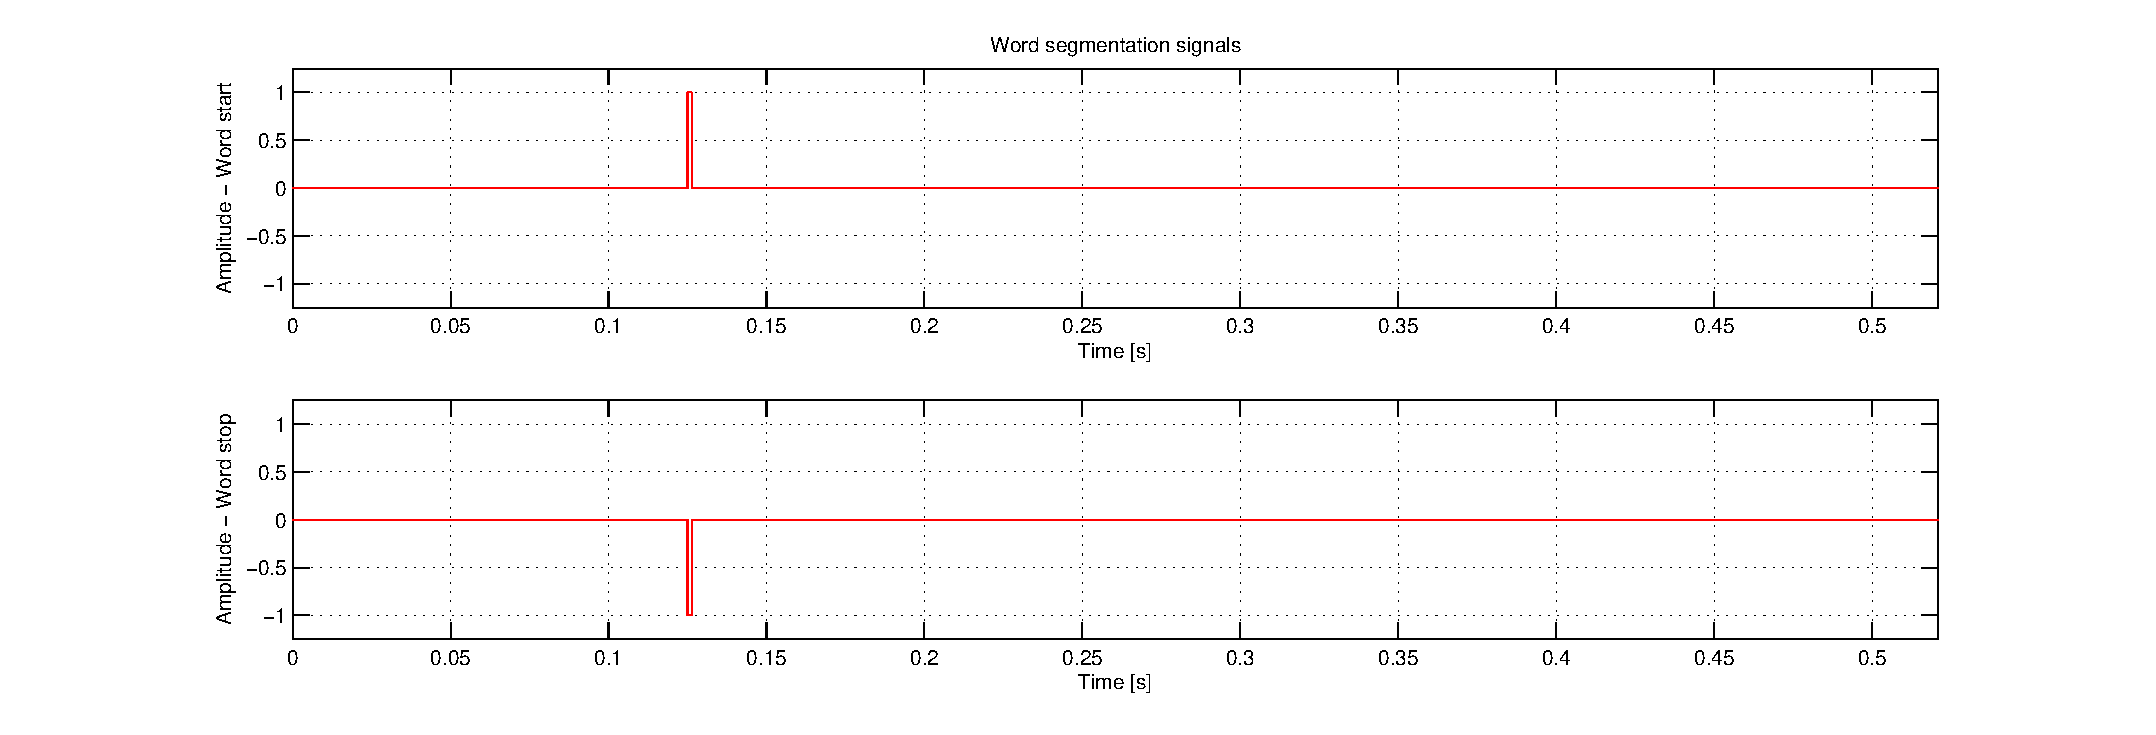
\includegraphics[width=\textwidth]{include/linguometer/images/seg_word.eps}}
	
	\caption[Segmentation signals]{\textbf{Segmentation signals}:
	the right channel component of the segmentation signals is shown (the left 
	channel has zero amplitude):
	(a) \emph{word batch start/stop} and (b) \emph{word start/stop}.
	The duration of the signals is 520 ms, while the duration of
	the peaks is 1.33 ms (64 samples). The first peak appears after 124 ms from
	the beginning of the tracks.
	In (a) the delay between two contiguous peaks is set to 124 ms. 
	Note: the amplitude axis interval is set to $[-1.50, 1.50]$ although
	the negative and positive saturation values are set to $-1.00$ and $1.00$
	respectively.
	The signals are stored in a Microsoft WAV container (PMC 16bit, 48kHz).
	}
	\label{fig:linguometer:architecture:sig:segmentation}
\end{figure}
% ---------------------------------------------------------------------------- %
